%%%%%%%%%%%%%%%%%%%%%%%%%%%%%%%%%%%%%%%%%%%%%%%%%%%%%%%%%%%%%%%%%%%%%%% 
%% 
%%
%% $Id: RoadMap.tex,v 1.19 2005/07/07 16:31:51 wmtan Exp $
%%
%%%%%%%%%%%%%%%%%%%%%%%%%%%%%%%%%%%%%%%%%%%%%%%%%%%%%%%%%%%%%%%%%%%%%%%

%%%%%%%%%%%%%%%%%%%%%%%%%%%%%%%%%%%%%%%%%%%%%%%%%%%%%%%%%%%%%%%%%%%%%%%
%% Specify basic document class and its options
%%
%% Use optional argument 'draftmode' to get the DRAFT watermark.

\newcommand{\docnumber}{}

\documentclass[draftmode]{memarticle}
%\documentclass{memarticle}

%\listfiles   % Uncomment this to write (in the log) the list of files used

%%%%%%%%%%%%%%%%%%%%%%%%%%%%%%%%%%%%%%%%%%%%%%%%%%%%%%%%%%%%%%%%%%%%%%%
% Document revision number, traced by using RCS revision number.
%
\RCS $Revision: 1.19 $

%%%%%%%%%%%%%%%%%%%%%%%%%%%%%%%%%%%%%%%%%%%%%%%%%%%%%%%%%%%%%%%%%%%%%%%
% Special macros for this document
%%
\newcommand{\Draw}{\productname{Draw}}
\newcommand{\Orca}{\productname{Orca}}
\newcommand{\Phedex}{\productname{Phedex}}
\newcommand{\Pool}{\productname{Pool}}
\newcommand{\Root}{\productname{Root}}
\newcommand{\Seal}{\productname{Seal}}

\newcommand{\EDFilter}{\classname{ED\-Filter}}
\newcommand{\EDProducer}{\classname{ED\-Producer}}
\newcommand{\EDProduct}{\classname{ED\-Product}}
\newcommand{\EDPid}{\classname{EDP\_id}}
\newcommand{\Event}{\classname{Event}}
\newcommand{\EventPrincipal}{\classname{Event\-Principal}}
\newcommand{\EventProcessor}{\classname{Event\-Processor}}
\newcommand{\FilterModule}{\classname{Filter\-Module}}
\newcommand{\FilterWorker}{\classname{Filter\-Worker}}
\newcommand{\Framework}{\classname{Frame\-work}}
\newcommand{\Getter}{\classname{Getter}}
\newcommand{\Mixer}{\classname{Mixer}}
\newcommand{\Module}{\classname{Module}}
\newcommand{\ModuleFactory}{\classname{Module\-Factory}}
\newcommand{\ModuleRegistry}{\classname{Module\-Registry}}
\newcommand{\OutputModule}{\classname{Output\-Module}}
\newcommand{\ProcessDesc}{\classname{Process\-Desc}}
\newcommand{\Provenance}{\classname{Provenance}}
\newcommand{\ParameterSet}{\classname{Para\-meter\-Set}}
\newcommand{\Path}{\classname{Path}}
\newcommand{\PluginManager}{\classname{Plugin\-Manager}}
\newcommand{\ProducerWorker}{\classname{Producer\-Worker}}
\newcommand{\PSid}{\classname{Para\-meter\-Set\_id}}
\newcommand{\RecAlgorithm}{\classname{Rec\-Al\-gor\-ithm}}
\newcommand{\RecCalibrationSet}{\classname{Rec\-Calibration\-Set}}
\newcommand{\RecConfig}{\classname{Rec\-Config}}
\newcommand{\ScheduleBuilder}{\classname{Schedule\-Builder}}
\newcommand{\ScheduleExecutor}{\classname{Schedule\-Exe\-cu\-tor}}
\newcommand{\Selector}{\classname{Selector}}
\newcommand{\Worker}{\classname{Worker}}

\newcommand{\DO}{D\O\xspace}

\newcommand{\order}[1]{$\mathcal{O}$(#1)}

%%%%%%%%%%%%%%%%%%%%%%%%%%%%%%%%%%%%%%%%%%%%%%%%%%%%%%%%%%%%%%%%%%%%%%%
%
% Document-specific parameters and settings:
%

\newcommand{\doctitle}%
  {CMS Core Software Re-engineering Roadmap}

\newcommand{\shorttitle}%
 {\doctitle}

\newcommand{\authors}%
  {
the EDM design team
%  K.~Bloom,
%  W.~Brown,
%  V.~Innocente,
%  C.~Jones,
%  J.~Kowalkowski,
%  L.~Lista,
%  M.~Paterno,
%  E.~Sexton-Kennedy,
%  W.~Tanenbaum,
%  L.~Tuura,
%and
%  A.~Yagil
  }

\hypersetup%
  { pdfauthor={}%
  , pdftitle={\doctitle}%
  , pdfkeywords={}%
  , pdfsubject={}%
  }

\tightlists

%%%%%%%%%%%%%%%%%%%%%%%%%%%%%%%%%%%%%%%%%%%%%%%%%%%%%%%%%%%%%%%%%%%%%%%
%
% Start the paper
%
%%%%%%%%%%%%%%%%%%%%%%%%%%%%%%%%%%%%%%%%%%%%%%%%%%%%%%%%%%%%%%%%%%%%%%%

\begin{document}
\topmatter

\chapter{Introduction}
\section{Purpose of this Document}

This document is a roadmap to aid the re-engineering of the CMS core software:
the \emph{event data model} (EDM) and \emph{framework}.
It contains many sections that are incomplete,
and will continue to do so for the foreseeable future.
It contains discussions of requirements,
system architectures,
design guidelines,
details of the design, and
plans for the future.

\section{Structure of this Document}

No section of this document is ``final''.
All are subject to change.

Sections marked \ldots
\begin{signednote}{Marc Paterno}
\ldots like this
\end{signednote}
\noindent
are notes added by one (or more) authors,
but that have not yet been ``approved'' as an official part of the document.
Section marked
\begin{fixme}
like this
\end{fixme}
are specially called out as incomplete sections.

Sections marked with like this: \\%
``\approved{7 Oct 1571}'' \\%
\emph{have} been officially approved.
This means that we consider the points in such a section settled.
In order to re-open such a point for discussion,
one needs to make a persuasive argument
that the related analysis is incorrect or incomplete,
and to persuade the others that some new analysis
is better.

In many parts of this document,
we refer to several examples
of code,
configuration information,
and other information.
While we strive to make the examples realistic,
we note that we are using them for expository purposes only.
We do not intend them to be taken a candidate physics algorithms,
or trigger algorithms.

\section{Scope of the Project}

The project includes two major sets of deliverables:
\begin{enumerate}

\item

a software framework for the creation of event-processing applications,
(called ``the framework'')
and

\item

a software framework for the representation
(both in-program and persistent)
of collider data,
both simulated and real,
(called ``the event-data model'',
or EDM).

\end{enumerate}

Included in this project
is the required mechanisms
to allow event-processing applications
to communicate with external systems
that perform the other tasks necessary
to allow efficient processing of event.

\begin{fixme}
Maybe we should put a list of these different systems,
or perhaps instead tasks,
here?
\end{fixme}

\section{Rationale for the Project}

\begin{fixme}
Put a statement of the reason for the re-engineering project here.
\end{fixme}

\chapter{Requirements}\label{ch:requirements}

We believe a loose definition of ``requirements'' is most useful.
We have not found it useful to make sharp distinctions between:
\begin{enumerate}

\item
\emph{constraints}, such as ``the code must compile with GCC 3.4.2'',
\item
\emph{behavioral} or \emph{functional} requirements,
\item
\emph{performance requirements}, such as
``the high-level trigger must accept $x$ events/s as input,
and produce $y$ events/s as output'', and
\item
\emph{software engineering guidelines}, such as the desire for testability.
\end{enumerate}

\section{``Physics Requirements'' from the CMS Computing Model}

\textbf{The CMS Computing Model}~\cite{CMSCM} specified 34 requirements
for the CMS Computing Model.
Some of these seem to be of direct relevance
to the design of the event-data model
and the event-processing framework.

\begin{description}

\item[R-1]
The online HLT system must create ``RAW'' data events containing:
the detector data,
the L1 trigger result,
the result of the HLT selections
(``HLT trigger bits''), and
some of the higher-level objects created during HLT processing.

\item[R-5]
Event reconstruction
shall generally be performed
by a central production team,
rather than individual users,
in order to make effective use of resources
and to provide samples
with known provenance
and in accordance with CMS priorities.

\item[R-6]
CMS production must make use of data provenance tools
to record the detailed processing of production datasets
and these tools must be usable
(and used)
by all members of the collaboration
to allow them also this detailed provenance tracking.

\item[R-13]
The online system
will classify RAW events into \order{50} Primary Datasets
based solely on the trigger path (L1+HLT);
for consistency,
the online HLT software will run to completion for every selected event.

\item[R-22]
A crucial access pattern,
particularly at startup
will require efficient access
to both the RAW and RECO parts of an event.

\item[R-23]
The reconstruction program should be fast enough
to allow for frequent reprocessing of the data.

\item[R-26]
CMS needs to support significant amounts of expert analysis
using RAW and RECO data
to ensure that the detector and trigger behavior
can be correctly understood
(including calibrations, alignments, backgrounds, \etc).

\item[R-27]
Physicists will need to perform frequent skims of the Primary Datasets
to create sub-samples of selected events.

\item[R-30]
Access to information stored in AOD format
shall occur through the same interfaces
as are used to access the corresponding RECO objects.

\item[R-31]
An ``Event directory'' system will be implemented for CMS.

\item[R-33]
Multiple GRID implementations are assumed to be a fact of life.
They must be supported in a way that renders the details largely invisible
to CMS physicists.

\item[R-34]
The GRID implementations should support
the movements of jobs
and their execution at sites hosting the data,
as well as the (less usual)
movement of data to a job.
Mechanisms should exist for appropriate control
of the choices according to CMS policies and resources.

\end{description}

\begin{fixme}
As other requirements from \cite{CMSCM} seem to be needed,
we can add them here.
\end{fixme}


Lacking from the list in \cite{CMSCM}
is a statement of the required \emph{speed}
of the high-level trigger.

\section{Constraints from Software and Computing Management}

Explicit processing path scheduling must be supported by this system;
the system must support the expression of data-flow paths within
job configuration. This feature will exist to support the trigger,
where users of the system directly state a path through which an
event will pass allowing resources to perform the task to be
estimated accurately at program start-up time.

\section{The CMS Analysis Model}

\begin{fixme}
What requirements to we have from the specification of the CMS Analysis Model?
What is the official reference that specifies the CMS Analysis Model?
\end{fixme}

\section{Requirements from the HLT}

\begin{fixme}
Put stuff here regarding how we want specification of high-level triggers
to be done as \emph{independent paths}, so that the designer of a trigger
doesn't have to understand other triggers.

It should also describe that we want the trigger program
to combine paths to allow for optimal execution.

We also require diagnosis of mis-configured trigger programs
at configuration (program start-up) time.
\end{fixme}

\section{Grid Computing Support}

The event-processing applications
need to be able to work in a grid environment.
While it is not always clear what this really means,
we understand it to mean
that an event-processing application
must expect to be ``packaged'' and sent to a target site.
The event-processing application must not make such packaging and submission unwieldy.

We do not expect the event-processing application
to directly support any particular ``grid technology''.
For example,
the event processing application will not itself submit remote jobs,
or request event-data files from remote resources.

\section{Several Typical Use Cases}

\subsection{Case 1: Official Jet Reconstruction with a Cone Algorithm}

\begin{fixme}
This is grossly incomplete; we'll add more as we understand what we need.
\end{fixme}

\begin{description}

\item[Task]

Jet reconstruction.

\item[Goal]

Use a cone algorithm to reconstruct jets,
starting from raw data,
putting the reconstruction results into the \Event.

\item[Actor]

Physicist who is running the event processing application
who wishes to run a specific cone jet algorithm.

\item[Precondition]

There already exists a file of events containing raw data.
The input and output configuration are already given
(and are outside the scope of this use case).

\item[Description]

\begin{enumerate}
  \item Make available parameter sets for the tower generating module,
        the cone jet algorithm, and the jet finder algorithm.
        We will build calorimeter towers from raw data,
        relying on an already-built vertex;
        Then we will build cone jets from these towers,
        recording full provenance information
        about the reconstructed information.
  \item Express in the task configuration that each of these modules
        is available
  \item Express in the task configuration that the Jets collection
        production is required
        (this assumes demand driven will be chosen for this job
  \item Identify the process to which this job belongs and the
        calibration/alignment set needs in the job configuration.
  \item generate a configuration bundle featuring all the above
        data
  \item use the identifier for the bundle to submit a job using
        an approved reconstruction executable
\end{enumerate}

\end{description}

\subsection{Case 2: Official Jet Reconstruction with a Cone Algorithm}

\begin{fixme}
Similar to case~1, but \emph{not} using official code---%
rather, using \emph{development} code,
and testing a new algorithm.
\end{fixme}

\subsection{Case 3: to be determined}

\begin{fixme}
More use cases can go here, if needed.
If not, the section title should be fixed.
\end{fixme}

\begin{fixme}
Insert a forward reference to \vref{sec:multipleproducts} here.
\end{fixme}

\chapter{Technology}

\begin{fixme}
Put here the technologies we must interact with.
For example:
\begin{itemize}
\item \Pool and \Root are to be used for persistency.
\item \Phedex is used for {\ldots} what?
\item {\ldots} lots of other products are used {\ldots}
\end{itemize}
\end{fixme}

\chapter{Architectural Overview}

\section{Responsibilities of Subsystems and External Systems}

The task of the event-processing application
is to process a sequence of collisions
(either simulated or real),
with the possibility of producing one or more output files.

\emph{Input modules} are responsible for obtaining events.
Each input module must understand one method of presentation:
\begin{itemize}
\item a sequence of event-data files, in the ``native format'' of the
application;
\item events presented to the high-level trigger as \ldots
\begin{fixme}
Put a description of how the raw data,
and the L1 data,
are presented to the HLT here.
\end{fixme}
\item
\begin{fixme}
What other presentation methods do we need? Events provided over a socket,
rather than a file? Does this even make sense? Are there others?
\end{fixme}
\end{itemize}

\begin{fixme}
What is the ``atom'' of event-data for file handling?
Are there any rules applied to decide whether two events can be in the same file?
What non-event data should be shipped \emph{in the file} with the event-data?
\end{fixme}

\section{Major Components of the Infrastructure}

The two major components of the core software are:
\begin{itemize}
\item the framework for the event-processing application, and
\item the event-data model.
\end{itemize}

\subsection{Architecture of the Event-Processing Application}

We will support two different ``styles'' of event-processing application
in the same software framework.
One style of application supports \emph{reconstruction on demand},
in the style of the previous \Orca framework.
The other style is more ``linear'',
and is more similar to the style
of the CDF and \DO
trigger and reconstruction frameworks.
We call these styles \emph{unscheduled} and \emph{scheduled}.

\subsubsection{Commonalities}

For both the unscheduled and the scheduled applications,
\EDProducer instances are the objects
that actually perform the task of reconstruction.
An author of an \EDProducer does not need to choose to support
one or the other style of use;
any \EDProducer is able to be used in either mode.

For both styles of application,
the same \EDProduct classes are used,
and the same \EDProduct instances will be produced
from identically-configured \EDProducer{}s.

For both styles of application,
the same parameter set system is used
to configure the \EDProducer{}s.

For both styles of application,
the same input and output formats are supported.

\subsubsection{The Unscheduled Application}

In the unscheduled application,
the action of requesting an \EDProduct
from the \Event
\emph{may} cause the invocation of an \EDProducer.
The high-level view of the mechanism is:
\begin{enumerate}

\item

User code requests an \EDProduct
through the \cppcode{Event::get}
member template,
possibly specifying a selector.

\item

The \Event looks for any already-created objects
of the correct type
(and that match the selector, if one was provided).
Such objects may be already loaded in memory,
or may be retrieved from the input source.

\item\label{i:find-edproducer}

If no match was found,
the \Event queries a registry of \EDProducer{}s
to discover which ones are able to create \EDProduct{}s
of the correct type
(and which could match the provided selector, if any).
If no such matches are found,
the user will receive an indication that no match
is available.
No new libraries can be loaded at this time.

\item

Any \EDProducer{}s found in step~\vref{i:find-edproducer}
are invoked,
creating their products
and entering them into the \Event,
and possibly causing a cascade of other reconstruction.

\item

Any \EDProduct{}s generated from the \EDProducer{}s
just invoked
are returned to the user.
If no appropriate producers were found,
no products may be returned.

\end{enumerate}

An unscheduled application is configured
by specifying:
\begin{itemize}
\item a selection of independent top-level \EDProduct{}s to be written out, or
\item a selection of independent high-level triggers to be run, or
\item an analysis module to be run, or
\item some combination of the above.
\end{itemize}
and also
\begin{itemize}
\item the menu of \EDProducer{}s that should be known
to the registry of \EDProducer{}s.
\end{itemize}

The combination of \EDProduct{}s in the input source
and \EDProducer{}s registered in the program
are the only things that limit the variety of \EDProduct{}s
than can be obtained from any \Event.

\begin{fixme}
What other useful ways are there to invoke an unscheduled application?
\end{fixme}

\subsubsection{The Scheduled Application}

A scheduled application is configured
by specifying a module instance path
through which the event will flow.
More derived or calculated products will be added
to the event as it moves through the path.

The responsibility of getting the proper dependency
ordering within an explicitly specified path lies
with person configuring the job.

\subsection{Architecture of the Event-Data Model}

\chapter{Analysis}

\section{There is more than one source of data}

Modules in an event processing application
obtain different types of data from different sources.
Conditions data come from services.
Geometry data come from services.
Event data,
and data related to collections of events
(such as \emph{runs} or \emph{luminosity blocks})
are passed to the modules
during the event processing loop.

\section{Templating or Base Class for \EDProduct{}s?}\label{sec:templatingorbaseclass}

It is possible to design the \Event and related classes
with either of two different different styles of design for \EDProduct{}s:
\begin{enumerate}\tightlist
\item \EDProduct{}s all inherit from a base class, or
\item \EDProduct{}s implement a simple generic programming \emph{concept}.
\end{enumerate}
In the first solution,
users writing their data classes must inherit from a base class;
in the second, there is no such need.
In both cases,
the ``get'' and ``put'' functions of the \Event
work with the user's class directly.

In the first solution,
heterogeneous containers of \EDProduct{}s work 
because all inherit from the base class \EDProduct.
In the second solution,
we'd have to introduce a base class,
and a ``wrapper'' template that inherits from it,
to form heterogeneous containers.
This wrapper would appear as another level of indirection
in the \Root output files,
at would be an (admittedly minor) annoyance to the user of the \Root prompt.

Solution two might allow use of simple things 
like \cppcode{std::vector<CaloJet>}
directly as an \EDProduct---except for the restriction noted below.
Solution one requires writing a class that could \emph{contain}
a \cppcode{std::vector<CaloJet>}.

We want every \EDProduct to know the \EDPid it is assigned.
Solution one allows this functionality to be supplied by the base class.
Solution two would require the \emph{concept} of \EDProduct to include
``getting'' and ``setting'' of \EDPid{}s;
thus \cppcode{std::vector<CaloJet>} would not be a suitable \EDProduct.

\section{Lifetime Management of \EDProduct{}s}

It is important that the lifetimes of the \EDProduct{}s
be controlled in a deterministic fashion,
to avoid resource leaks.

Because the persistent format of the CMS data
is based on \Root,
we considered having the \EDProduct instances
allocated directly in \Root buffers.
While this has the beneficial feature of avoiding
a memory-to-memory copy of the \EDProduct,
it has several drawbacks that made us decide to \emph{not} choose this design.
The drawbacks we identified are the following.
\begin{enumerate}

\item

It makes a stronger coupling between the \EventPrincipal and \Root.

\item

This couping makes it much harder to create \EDProduct instances
that will \emph{not} be managed by \Root.
This may be important for the high level trigger,
which will process many events that are rejected.
Creating and destroying objects in \Root buffers,
and the detailed management necessary to avoid corruption of the files created,
may waste critical time in the trigger.

\item

This coupling would make it much harder to write the same event-data
to several different outputs,
whether those outputs are multiple \Root files
or output formats \emph{other} than \Root.

\item

This coupling may make the writing of selected
(rather than \emph{all})
\EDProduct{}s in an event
to persistent storage.

\end{enumerate}

For these reasons,
we believe that the cost of a memory-to-memory copy
of those \EDProduct{}s selected for output
is less than the cost of the design that avoids that memory-to-memory copy.

\section{Unambiguous identification of reconstruction results}

It is critical for users to be able to unambiguously identify
how each reconstruction result was produced.
There are several varieties of information that constitute this
identification.

Collectively,
we refer to all this information as the \emph{provenance}
of the \EDProduct.
Each \EDProduct is associated with a \Provenance object
that records this information.
Where appropriate,
\Provenance objects are shared between \EDProduct instances.

\begin{enumerate}

  \item Module configuration

  \begin{enumerate}

    \item

    The unique identifier representing all (the names and values)
    of the run-time configuration parameters given to the module.

    \item

    A string giving the fully-qualified class name
    of the module.

  \end{enumerate}

  \item Parentage

  A vector of the unique identifiers of the \EDProduct{}s used
  as inputs for this bit of reconstruction.

  The identifiers are unique to the event. It is possible to 
  maintain common identifier lists and tag those with an ID
  and only record.

  Although
  a module can make use of more than one input to create its output,
  we make no attempt to specify the \emph{type} of the \EDProduct
  to which each of the entries in this vector refer.
  If such identification is needed in a particular \EDProduct,
  that product can store the information in its own member data.
  We rejected
  providing a \emph{mapping} of class name to
  \EDPid
  because we deemed the complexity unwarranted for the simple use
  to which the ``parentage'' information,
  in this general form,
  is put.
 
  \item Executable configuration

    \begin{enumerate}

    \item

    A ``human friendly'' string called a module label, which is
    a unique identifier (within a job) used for \EDProduct{}s 
    created by the module
    configured by this label.
    This label comes from a module configuration
    parameter with a fixed name.
    Each module has exactly one of these.

    The label configuration parameter is special.
    Changing the label in the configuration will cause a new 
    module to come into existence because a unique ParameterSet
    determines module instances.  However, the label is not
    part of the permanently generated ID.

    \item

    A single version number
    that defines the code
    for the entire executable.
    The user can obtain specific library version numbers
    by querying a central database,
    using this version number.

    The value is only meaningful for tagged releases.

    This number specifies which libraries
    were \emph{available} when building the application;
    it does not indicate that \emph{all} such libraries were used.
    \end{enumerate}

  \item Conditions Data

    An identifier representing the calibration and alignment set
    that was used in the construction of this \EDProduct.

    We assume here that calibration and alignment are handled in the
    same way and that this single, high-level identifier refers to all the
    calibration information used for this event. It is possible that
    individual calibrations (\eg silicon, calorimeter, muon) will also
    have IDs associated with them and that each of these will need to
    be recorded instead of the ``set'' ID.

    Other conditions data IDs may also be needed here, such as
    geometry version or hardware configuration.

  \item Job configuration

    A physical process name.  A job starts up in a particular context
    such as HLT or Reconstruction. This name identifies the process
    under which the job was started and is likely to be a run-time
    property.

    \begin{fixme}
    A pass identifier?
    \end{fixme}

\end{enumerate}

All of this provenance data is distinguished from the event
data because its principal home is in an ancillary database,
although a copy may be readily accessible from the event data
(\eg within the file that contains events).

\section{Branch naming from provenance information}\label{sec:branchnames}

Provenance data will exist in a form that is traversable from
the \Root prompt (browsable).

The branch name is composed of a 
  \begin{enumerate}\tightlist
  \item Friendly product type name
  \item Process name
  \item Module label
  \end{enumerate}
The separator is assumed to be an underscore.
Friendly product type name comes from the persistency tools.
Its definition is assumed to be external to the source code and
module configuration system.
The provenance will not maintain this string.

This will help users move between the ``data'' and \cpp object model
views of the EDM.

\section{Communication between event-processing elements%
\label{sec:communication}}

\approved{7 March 2005}

Clearly the event-processing elements (called here \emph{modules})
need to communicate---%
the hits produced by one module will be used to form tracks by another.
In order to provide for modular testing,
which is important for quality assurance of the physics results,
we require that modules communicate \emph{only} through the \Event,
by putting \EDProduct{}s into the \Event.
Furthermore,
we require that one may ``cut'' the event-processing chain 
between any two modules,
and save the state of the event at that instant.
This requires that all \EDProduct{}s be \emph{persistable}.

While each \EDProduct must be persistable,
this does not imply each one must be persisted
for every event.
The event output mechanism must be capable
of selective writing of \EDProduct instances,
for example to several output streams.

We recognize the fact that placing this requirement
on the design of all \EDProduct{}s
makes the burden on the designer of each \EDProduct class
at least slightly greater.
It is important for us to keep this burden as small as possible,
without violating our other requirements.

\section{Input is Not Like Output}\label{s:inputandoutput}

There is a lack of symmetry between input and output of events.

In the context of several paths of execution,
it is possible to schedule output
perhaps to multiple streams
in each path of execution.
For example,
a single event processing executable
might contain a path performing $W$ mass analysis,
and a second path performing $t\bar{t}$ mass analysis.
Each of these paths could usefully write those events interesting to the analysis
to its own stream.

Input of events does not have such a similar use.
Each job has a single ``driving source'' of events.
This source might read several files,
perhaps in parallel.
The input still appears to the event processing application
as a single stream of events.

For these reasons,
we see the need for an \emph{input service},
which is not a module,
and for \emph{output modules}.

In general,
the framework will invoke the appropriate input service.
As a special case,
a \emph{mixing module} could invoke
an additional input service or services.

\section{Event mixing module}

\subsection{Use cases}

\subsubsection {Use case 1}

Merge Hits from a number of pileup simulated events to a signal simulated event.

The number of pileup events to be merged is a function of the machine luminosity.
Out of time pileup must be considered in addition to in-time pileup. The number of crossings before and after the nominal one to be considered is sub detector dependent.

This is the main use case, and is needed for the digitization of simulated data in the new framework.
This use case has a production flavor.
\subsubsection {Use case 2}

Merge a signal event to another signal event, to simulate more complicated events.

Ex. merge single electron event on top of a jet QCD event to study electron id,..This is a use case with analysis flavor. \\
Do we need here to consider also the case of mixing events from real data?

\subsection {Requirements}
\begin {itemize}
\item
the software must fit into the new EDM requirements

\item
there is an I/O efficiency requirement, at least for us ecase 1. Considering out-of-time pileup from -5 bunch crossings and up to +3 bunch crossings and the highest luminosity giving ~17.5 pileup events in average per crossing, this gives a number of ~160 pileup events as input to be merged to a single signal event. Typical size of pileup events at Hit level is ~150kB, and ~500kB for signal events.
That means that the mixing module must be able to handle ~25MB of input and 0.5MB of output in a 
very short processing time.
\item
Fixed, HIC and Poisson are different possibilities to define the number of pileup events to mix. All of these should be implemented.
\item
configurability: things like the number of bunch crossings to be considered must be configurable differently for each subdetector. But for use case 1, flexibility may be very limited, whereas for use case 2 more configurability might be needed.
\item
MC true information must be accumulated. A minimum requirement is that entering particles are kept, and that a distinction between signal and pileup is made.  More requirements may be desirable.

\item
Do we need to maintain/ensure consistency between the mixed events? Is it allowed/useful to mix any event with any other?

\end {itemize}

\subsection {Random sequence for pileup mixing}

We assume that pileup events have been randomly generated. Since the pileup 
sample has finite statistics, one has to generate many sequences of 
(up to ~160) pileup events from a finite collection of events in order to 
produce as many independant sequences as possible. Since the event collection 
is finite, events have to be reused in several sequences (for a 1M pileup 
event size and for high luminosity, events will be reused starting in 
average from at most the 57143th sequence). In addition, for efficiency 
reasons, it is highly desirable to limit as much as possible jumps into new files.

\subsection {Mixing module in new framework ({to be completed})}.

Since the mixing module producing products for writing to the EventStore, it will
be a EDProducer.  But it is different from normal Event processing modules because it is 
not driven by a single source of events, but by two input streams.

\subsubsection {Demands on the input service}
A specific method of the input service will be needed, allowing to get a vector of events 
the length of which has been specified by the caller. Depending on the possibilities of 
randomness desired when selecting pileup events, it might also be necessary to specify 
in detail how and with which configuration the pileup events are selected.

\begin{fixme}
This list is very incomplete.
Please add additional items you think are needed.
\end{fixme}

\section{Schedule Specifications for the HLT}

This section describes rules regarding module scheduling and
configuration within the HLT.

\subsection{Concept Definitions}
\begin{description}

\item[Reconstructor]

A module whose primary purpose
is to perform some step of reconstruction
and to place the result into the \Event.

\item[Filter]

A module whose primary purpose
is to render a decision on the quality of an \Event,
based on the \EDProduct{}s in the \Event.

\item[Path]

The user's expression
of requirements
regarding which modules
(including their configurations)
make up a single high-level trigger.

\end{description}

\subsection{Example Problem}

\begin{fixme}
The English description of the problem should go into the use cases section.
\end{fixme}

We consider the problem setting up a HLT program using two triggers:
\begin{enumerate}
\item a top--muon trigger ($t_\mu$), which looks for a high-$p_T$ muon and several jets, and
\item a top--electron trigger ($t_e$), which looks for a high-$p_T$ electron and several jets.
\end{enumerate}

The $t_\mu$ trigger uses jets from the midpoint cone algorithm,
and the $t_e$ trigger uses jets from the $k_T$ algorithm.

\subsubsection{\texorpdfstring{Top (muon) trigger: $t_{\mu}$}{Top (muon) trigger}}

This trigger requires tracks from a specific algorithm (module $B_1$),
which in turn requires unpacking the tracking raw data (module $A$).
It also requires jets from the midpoint cone algorithm (module $D$),
which in turn requires unpacking calorimeter data (module $C$).
Finally, it requires muons (module $F$), made using tracks from $B_1$.

\subsubsection{\texorpdfstring{Top (electron) trigger: $t_{e}$}{Top (electron) trigger}}

This trigger requires tracks from a specific algorithm (module $B_2$),
which in turn requires unpacking the tracking raw data (module $A$).
It also requires jets from the $k_T$ algorithm (module $E$),
which in turn requires unpacking calorimeter data (module $C$).
Finally, it requires electrons (module $G$),
made using tracks from $B_2$ and the calorimeter data from $C$.

\subsection{An Insufficient Solution}

A simple solution to this problem
would be to have the user specify each independent trigger
by specifying the sequence of modules to be run,
in the order in which they are to be run:
\begin{itemize}
\item $A \rightarrow B_1 \rightarrow C \rightarrow D \rightarrow F$ for $t_\mu$
\item $A \rightarrow B_2 \rightarrow C \rightarrow E \rightarrow G$ for $t_e$
\end{itemize}

This solution is inadequate
because it does not convey important information that the user knows
and that could be used to compute an optimal schedule.
In the case above,
this information is that the calorimeter-based modules ($C$, $D$ and $E$)
are independent of the tracking-based modules ($A$, $B_1$, $B_2$ and $F$).
Because they are independent,
the ordering of the calorimeter-based software
and the tracking-based software
implied by the sequences above
are not essential.
Only the ordering \emph{within} the tracking set,
or the calorimeter set,
is essential.

\subsection{A Sufficient Solution}\label{sec:hltgrammar}

The critical observation is that each trigger description
(such as those above)
can be composed from strictly linear sequences
that are independent of each other,
and that can be combined to produce the full trigger specification.

We see the need for a configuration language
richer than the simple one above,
that allows specification of:
\begin{itemize}

\item
(optionally named) sequences of configured modules,
which the schedule builder may \emph{not} re-order,
(because of implied dependence of later modules on
the output of the earlier modules), and

\item
combinations of (optionally named) independent sequences,
with no implication regarding the relative order
of the constituent sequences.

\end{itemize}

Furthermore,
we want the elements of a sequence to be either individual modules,
or the combinations of independent sequences.

Finally,
the schedule builder must be able to read a configuration 
of the trigger program
written in this language,
and to perform ``optimizations'' that do not
change the meaning of the program,
but that avoid redundant execution of any module.

We can capture the essential features
of this configuration language
via the grammar in Figure~\vref{fig:config-grammar}.
The sequence operator ``,'' is used to express dependencies between modules.
It has higher precedence than the \& operator,
which is used to combine the results of independent sequences.
\verb!'ConfiguredModule'! are terminal symbols
in this grammar.
\begin{figure}[h]
\begin{verbatim}
TriggerTerm    ::= PathExpression

PathExpression ::= PathExpression & Sequence
                 | Sequence

Sequence       ::= Sequence , ProcessingUnit
                 | ProcessingUnit

ProcessingUnit ::= 'ConfiguredModule'
                 | ( PathExpression )
\end{verbatim}
\caption{The configuration grammar for scheduled event-processing applications.}
\label{fig:config-grammar}
\end{figure}

A trigger job will consist of many of these \emph{TriggerTerm}s.

\section{Multiple Products from One \EDProducer}\label{sec:multipleproducts}

Many problems are arising
when we consider allowing multiple objects of the same type
to be produced by a single \EDProducer.
The source of the problem
is the fact that the produced objects
are distinguishable neither by
type
nor by
provenance (which describes the configuration
of the producer
and the ``context'' in which the producer was run).
Thus,
to distinguish between multiple objects of the same type
produced by a single \EDProducer,
one is forced to look at
the data of the \EDProduct itself.

The problems include:
\begin{enumerate}

  \item   
  Schedule validation becomes difficult.
  It seems to require creation of prototype instances
  of the \EDProduct{}s at configuration time,
  so that the relevant data can be matched
  (by a \Selector that knows about that specific
  \EDProduct).

  \item  
  The need to create these prototype objects
  limits our flexibility in having \EDProducer{}s
  announce what they make.

  \item 
  It requires that we support \Selector{}s that look
  at \EDProduct{}s (and concrete subclasses),
  not just \Provenance{}s.
  This puts a greater demand on the authors
  of \EDProducer{}s and \EDProduct{}s
  to create the relevant \Selector{}s.
  Previous experience leads us to believe
  it will be difficult to assure all
  \EDProduct designers
  will produce the appropriate \Selector classes.
\end{enumerate}

We propose that \Selector{}s
passed to the \Event should only operate on
\Provenance{}s.

When combined with the requirement
that \EDProducer{}s
use only the \cppcode{Event::get} function
that returns a single \EDProduct,
there is a drawback to this choice.
It means that \EDProducer{}s
can not make use of the output of 
other \EDProducer{}s that make multiple instances
of the same type.
We propose that the solution for this
is for the \Provenance to carry
a user-supplied bit of data
that can then be used by the \Selector
to identify a single matching \EDProduct.
However, we expect this to be a rare case.


\section{Access to \EDProduct{}s}\label{sec:access}

\subsection{Definitions}\label{sec:accessdefinitions}

\begin{description}

\item[Event]

The \Event is an interface through which one gains access
to detector output 
and derived quantities that are associated with a \emph{single collision}.

\item[Selector]

A \Selector is a predicate 
used to identify interesting \EDProduct{}s.
It does so by examining the \Provenance
associated with that \EDProduct.
It encapsulates the user's requirements 
(\eg features of interest) for products.
The typical use case will be to have a \Selector examine a single feature and then through composition and more complex \Selector can be created.

\item[Provenance]

A \Provenance carries a snapshot of
the data relevant to describing how an \EDProduct
was built.
It includes (but is not limited to):
\begin{enumerate}

\item Description of the configuration of the module
that made the \EDProduct.

\item Description of the program configuration
    (\eg code version).

\item Parentage of the \EDProduct
(\ie what other
\EDProduct{}s were used as ``inputs'' by the
\EDProducer that made the \EDProduct).
\end{enumerate}

Note that some, 
but not all,
of this information is available
at program configuration time.

\item[Getter]

A \Getter provides an interface through which a \emph{single}
\EDProduct is obtained.
\end{description}

\subsection{This needs a home nearby}

\begin{fixme}
A note concerning selectors:
In order to make selectors friendly to use,
several standard selectors are necessary.
A special GetLatestCreated
(implies that the order of creation is maintained).
The list used by this selector,
is maintained as file-level metadata.
\end{fixme}

\subsection{Guidelines}

We believe the following guidelines are important:
\begin{enumerate}

  \item
  It is convenient to allow human-readable strings
  (labels)
  to be used in the identification of \EDProduct{}s.

  \item
  It is critical that access using any such strings
  never anything other than a single \EDProduct.

%  \item
%  It is critical that any such strings
%  unambiguously identify a \emph{single} \EDProduct,
%  and that the software guarantee the one-to-one mapping.

  \item
  Access to \EDProduct{}s must be type-safe,
  and so they must specify the (\cpp) \emph{type} of \EDProduct
  to be returned.
  Allowing the user to obtain all objects of a type
  that derive from a common specified type
  would complicate the interface for doing so.
  We believe such use would be rare.

\end{enumerate}

See also \S\vref{sec:branchnames} on branch naming,
which touches on related issues
regarding string labels.

\subsection{Anticipated Access Needs}

We the following access methods are important.
The order below does \emph{not} imply an order of importance.
In each example below,
the query supplies the type of \EDProduct
to be retrieved.
This is only a representative sample,
not an exhaustive list.

\begin{enumerate}

\item
Return handles to all \EDProduct{} objects of a given concrete type.
This can return multiple handles.
If no objects are found, throw an exception.

\item
Return a handle to the one \EDProduct object that has a given \EDPid.
If there is none, throw an exception.

\item
Return a handle to the \EDProduct of a specific type,
made by a particular reconstruction module,
giving the full specification of the module's configuration.

\end{enumerate}

In addition to these basic queries,
we also need to support ``modifiers'' for queries---%
that is,
the ability to select the \EDProduct{}s to be returned
by logical ``and''-ing of the queries above
with the following additions.

\begin{enumerate}

\item
Restrict the \EDProduct{}s returned by specifying a 
``process name''.

\item
Restrict the \EDProduct{}s returned by specifying a
``release number''.

\item
Restrict the \EDProduct{}s returned by specifying some
part of the \Provenance information that must also be matched---%
for example, to obtain all the results of midpoint-cone jet algorithms,
disregarding the remaining details of the configuration information.

\item
Return the \EDProduct{}s returned 
by specifying some feature (a value or range of values)
of a parameter in the \ParameterSet of the product's \Provenance.
For example, to obtain all the results of midpoint-cone jet algorithms
that have a cone radius between 0.5 and 1.0.

\end{enumerate}

Note that many \EDProduct{}s contain \emph{collections} of objects, 
\eg tracks, jets, or muons.
The \Event interface only supports obtaining \emph{entire} \EDProduct{}s.
It does \emph{not} directly support 
obtaining subsets of elements
contained within and \EDProduct.

\subsection{Proposal}

We propose that \EDProduct{}s should be accessed only through the \Event.

We propose that all access methods will ``match'' 
only the \emph{most derived type} of the \EDProduct requested---%
that is,
the type must be an exact match,
not a match to a base class.
One can not make any single ``get'' to obtain
all \EDProduct instances
of types that derive from a common base.

We propose the \Event has three member templates
for retrieving \EDProduct{}s.
Each is parameterized on the type of the \EDProduct to be retrieved.

\begin{enumerate}

\item 
\cppcode{get} takes a \Selector object
and returns the single \EDProduct
that has \Provenance
that matches the \Selector.
If there is not exactly one such match
this \cppcode{get}
throws an appropriate exception.

\item
\cppcode{getByLabel} takes a string label
and returns the unique \EDProduct
of the appropriate type
with a \Provenance with the matching label.
If there is not exactly one such match
this \cppcode{get}
throws an appropriate exception.

\item
\cppcode{getMany} takes an optional \Selector
and returns all the \EDProduct instances
of the appropriate type
that match the \Selector,
or all the ones of the appropriate type if no \Selector is specified.
\EDProducer{}s shall not use \cppcode{getMany}.

\end{enumerate}

\subsection{Consequences}

We propose that the \ParameterSet that configures an \EDProducer
must have a string parameter named ``label''.
This will the the unique label assigned to every \EDProduct
created by the \EDProducer instance
configured with that \ParameterSet.

At module configuration time,
the uniqueness of these labels---%
for \EDProduct{}s to be created by the current program---%
will be verified.


Because it is possible for the input file
to contain \EDProduct instances
with labels that will collide with those of \EDProduct{}s
to be generated in the current program,
the system must have a way to deal with such collisions.

We propose that an attempt to insert a new \EDProduct with label \textit{x}
into an \Event that already contains an \EDProduct of that type and label \textit{x}
result in an exception throw.
This assures that the \Event never gets into a state
in which it contains two \EDProduct{}s
of the same type
that have the same label.

In order to make it easy for users to run a reconstruction program
that replaces ``old'' versions of some \EDProduct
with ``new'' versions of those \EDProduct,
we propose there exist an ``\EDProduct dropping module''.
This module should be user-configurable,
so that it is easy for the user to specify which \EDProduct{}s
are \emph{not} to be read from the input.
This does \emph{not} imply that all \EDProduct{}s must be read from disk on input.
Rather, it is possible that this ``module'' work by indicating to the file-reading mechanism
that a given \EDProduct ``branch'' is to treated is if it did not exist.

\begin{signednote}{Marc and Jim}
We think the rest of this section should be removed.
\end{signednote}

There is more than one variety of event query.
\begin{itemize}

\item 

In \EDProducer{}s,
the query functions
can return only exactly one product.
If the requested product can not be returned,
and exception shall be thrown.

\item

In an analysis module,
an addition query interface is available.
These queries may return multiple matching products.

\begin{fixme}
We have not decided what happens if a failure during reconstruction occurs.
How does the data indicate that an algorithm was tried,
but failed to complete?
Perhaps we can make the \Root branch entry
contain a 2-tuple,
consisting of the constructed object (if any)
and an error report object (if any).
Only one of the two items would actually appear
in any entry.
\end{fixme}
\end{itemize}

\section{Insertion of \EDProduct{}s}\label{sec:insertion}

See \S\vref{sec:accessdefinitions} on page~\pageref{sec:accessdefinitions}
for the definitions of important terms in this section.

The question we answer here is: What code
developers of  \EDProducer{}s write
to put the \EDProduct{}s they create
into the \Event?

We have two proposals,
and need to select which one we will choose
for further design.

\subsection{Solution One}

Data products are allocated
and inserted
through the \Event.

The \Event contains a \cppcode{put} member template.
\cppcode{put} is parameterized on the type of \EDProduct
and is used to allocate an object
that will automatically be placed permanently into the \Event
when the \EDProducer successfully completes its task.

Each \EDProducer that make more than one \EDProduct
will invoke \cppcode{put} for each of the \EDProduct{}s it generates.
All the \EDProduct{}s will be successfully added to the \Event,
or none will be added.

A \Provenance object is added 
to the \Event
by the framework
during the final commit.
The user is not responsible
for handling this information.

The main goal of this solution
is to mimic the procedural model
that we (Jim and Marc) have observed
to be the favorite of 
most authors of reconstruction code.

\subsection{Solution Two}

\EDProduct{}s are allocated dynamically
and returned by the \cppcode{produce} method of the \EDProducer.
Ownership of the created products is passed during the return.

The framework handles inserting the created products
into the \Event.
A \Provenance object is added automatically
by the framework.
The user is not responsible
for handling this information.

The main goal of this solution
is to allow the system to determine,
at compile time,
what \EDProduct types
are created by a given \EDProducer
by working with the return type
of the \cppcode{produce} function.

Thus the function type of \cppcode{produce}
is different for each kind of \EDProduct.

\subsection{Comparison}

Solution~1 has ``parallelism of interface''.
The user's model of the \Event
as repository of \EDProduct{}s
is respected:
a user obtains input \EDProduct{}s directly from the \Event
and inserts newly made \EDProduct{}s directly into the \Event.
Solution~2 lacks this parallelism.

In Solution~1,
the transactional model is less obvious
for \EDProducer{}s that make more than one \EDProduct instance.
The user's code might have the \cppcode{put}
for the two \EDProduct{}s
widely separated.
In Solution~2,
the two objects are clearly returned together.
Since the transactional model
assures that \emph{both} are committed
or \emph{neither} is committed,
the behavior in both cases is the same.

The \Event is already a heterogeneous collection of \EDProduct{}s.
In Solution~1,
we make use of this directly in the interface of the \Event
for both all \cppcode{get} templates and for \cppcode{put}.
In Solution~2,
we do not benefit from this,
because the user does not put results directly into the \Event.
We see two different paths to follow:
\begin{enumerate}
\item
Introduce a second heterogeneous collection of \EDProduct{}s
to be the return type of the \cppcode{produce} function,
so that each function can have the same return type.
This seems to violate the purpose of Solution~2,
since it is no longer possible to deduce the type of the returned \EDProduct{}s
from the type of the \cppcode{produce} function.
\item
Introduce several member templates
(\eg \cppcode{produce}, \cppcode{produce2}, \ldots),
each of which has a different return type.
\end{enumerate}

We expect that most \EDProducer{}s 
will insert a single \EDProduct
into the \Event.
Complicating the mechanism by which this is done
for the common case,
in order to support the rare case of multiple insertions,
is a disadvantage.

\section{Comparison of the \RecAlgorithm System to \EDProducer{}s}

In this section,
we compare the initialization
of \EDProducer{}s
and \RecAlgorithm{}s.

\subsection{What is an ``algorithm''?}

In the \RecAlgorithm system,
an algorithm objects are
``entities that create new resulting objects or transform input objects''.
Algorithms in general
\begin{itemize}\tightlist
\item have a state (or configuration),
\item have some inputs, some of which are the results of other algorithms.
\end{itemize}

In the \EDProducer system,
we distinguish between
\begin{itemize}
\item \EDProducer{}s, 
the top-level, 
reconstruction-developer written,
framework components
that perform a quantifiable step of reconstruction,
by creating and storing persistable data in the \Event, and

\item the much looser category of ``algorithms'',
that can perform smaller steps of reconstruction,
and that may be composed to form an \EDProducer.

\end{itemize}

The \EDProducer system has no formal notion of ``algorithms''
as components;
the author of an \EDProducer
is free to use any internal organization suitable for his task.

\subsection{Who are the ``users''?}

We find it useful to distinguish between two groups of ``users'':
\begin{itemize}\tightlist
\item (algorithm) \emph{developers}, who write reconstruction code
(but are users of the core infrastructure), and
\item \emph{end users}, who configure and run an event-processing
program.
\end{itemize}
Of course, an individual may play both roles, at different times.

\subsection{Coupling of algorithm system to configuration system}

In the \RecAlgorithm system,
the algorithmic objects
are tightly coupled 
(though inheritance of implementation)
with the parameter set (and other configuration)
objects.
It is not possible to make use of an algorithmic object
without the presence of the full configuration system.

In the \EDProducer system,
an ``algorithmic object''
(\ie a component with an \EDProducer)
does not need to have
any interaction at all with the \ParameterSet object,
nor with the rest of the parameter set system.
The algorithm developer is free to decouple the algorithm
objects from the parameter set system, if he so wishes.
Because the \ParameterSet system
allows nesting of \ParameterSet objects
to arbitrary depth,
the developer is free to make use of \ParameterSet{}s
in configuring nested algorithms.

\subsection{Algorithm names}

In the \RecAlgorithm system,
each algorithmic object has a developer-assigned name;
the examples show these names compiled into the code.
The scope of these names is the entirety of \Orca;
each algorithm name must be unique within this scope.

In the \EDProducer system,
the approximate equivalent to this algorithm name
is the combination of \EDProducer \emph{class name}
and \emph{instance label}.
The class name is of course unique within any program.
The scope of an instance name
is a single running process;
the name must be unique within that scope.
The instance label is a configurable parameter
assigned (by the end user) 
at runtime.
See elsewhere in this document for the use of the instance label.

\subsection{Version identification}

In the \RecAlgorithm system,
each algorithmic object has a version identifier,
expressed as a string
assigned by the algorithm developer
in the code.

In the \EDProducer system,
the approximate equivalent
is the CVS tag for the entire code-base
used to construct a release;
this is provided automatically,
and is recorded in the created event data.

Developer-updated version information
may be neglected by the developer,
and is not certain to be of the ``accepted format''.
Enforcement of standards is left up to inspection of releases.
Automatic handling of the version updating can not be neglected,
and is assured of uniformity.

\subsection{Types of parameters}

In the \RecAlgorithm system,
the \ParameterSet supports
types 
double, int, string, and bool.
Additionally,
the \RecConfig
that contains a \ParameterSet
can also contain additional \RecConfig{}s.

In the \EDProducer system,
the \ParameterSet supports
these types, 
as well as vectors of these types.
This \ParameterSet also directly supports
nesting of \ParameterSet{}s,
and vectors of \ParameterSet{}s.

\subsection{Handling of \cppcode{double}s}

In the \RecAlgorithm system,
each parameter of type double
is associated with a \emph{tolerance}.
Such parameters are compared for equality
using their tolerances.

In the \EDProducer system,
parameters of type double
are compared directly.
Note that such parameters are read,
written, and compared---%
they are not used in calculation,
and so no troubles with inexact representation
of calculated quantities arise.

We note that
use of tolerances in ``equality'' comparison
cause the ``equality'' comparison to fail to satisfy transitivity.
Failure of transitivity may lead to unexpected results.

\subsection{Default parameters for algorithms}

In the \RecAlgorithm system,
each algorithmic object
is required to have
a default value 
for each parameter
compiled into the source code.

In the \EDProducer system,
to aid in tracing the behavior of reconstruction,
default values of parameters
compiled into the source code
are expressly forbidden.

\subsection{Calibration data in algorithm configuration}

In the \RecAlgorithm system,
one of the parts of a \RecConfig object
is a \RecCalibrationSet.

In the \EDProducer system,
calibration data are not considered to be part 
of the algorithm configuration system.
They are handled as separate problems,
and are decoupled.


\chapter{Design of the Core Infrastructure}\label{chap:infrastructure}

\section{Overview}

The main elements of the core infrastructure are:
\begin{enumerate}
 \item the classes \Event and \EventPrincipal,
 \item the ``module'' base classes \EDProducer, \EDFilter, 
       \Mixer, and \OutputModule,
 \item the classes \ScheduleBuilder, \ScheduleExecutor,
       and the variety of ``worker'' classes,
 \item the \ParameterSet class and its related classes,
 \item the \Framework class.
\end{enumerate}

\section{The \Event}\label{sec:event}

There will be only one \Event class.

Purpose: Responsible for managing lifetimes for each \EDProduct{}
it contains. Manages relationships between \EDProduct{} and metadata.  Provides
access to event data (\EDProduct{}s) for any consumer of event data.  Allows
communication between ``modules.''

A single \Event{} instance corresponds to the detector output, reconstruction products, and/or
analysis objects from a single crossing or the simulation of a single crossing.

\Event{} is a concrete class.

It is possible to allow different \Event{} interfaces, or merely different member functions,
some of which perform ROD, and some of which do not.
\begin{itemize}
 \item
   Any \EDProduct{} should be immutable after insertion into the \Event{}
   (see \S\vref{sec:rulesforedproductmodification}).

 \item
   The \ParameterSet provenance of input objects to a particular
   \EDProduct{} should survive the dropping (\emph{dropping} means
   not writing to the output file) of the original input object.
\end{itemize}

The \Event{} will use methods of the \Selector{} class (see \S\vref{sec:selector}) to search for
\EDProduct{}s matching a given criterion.

An ancillary class of the \Event{} will keep track of the full
invocation sequence
\begin{enumerate}\tightlist
\item \cppcode{EDProducer::produce},
\item \cppcode{Event::make},
\item \cppcode{Event::get}.
\end{enumerate}
This information will be used to
build a provenance ``record'' to be associated with the \EDProduct.

\section{\EDProduct{}s}

Purpose: The basic unit of event data managed by the \Event{}.

\EDProduct{} is the base class for all objects inserted into the \Event.
Derived classes are also referred to as \EDProduct{}s.
Each instance of such a class represents a component of an event,
and must be capable of persistence.

Each \EDProduct{} instance has an ID that is unique within the \Event,
and which is assigned by the \Event
during its insertion into the \Event.

A ``map'' of the \EDProduct{} instances for an event is kept in the event store.

\begin{signednote}{Luca Lista}
Using a generic approach may shield the end user from exposure to
the \EDProduct{} class, allowing the use of any type, not only
\EDProduct{} subclasses. This is done, for instance, in BaBar
using the \classname{ProxyDict} technique~\cite{ProxyDict}.

For ``bare root'' access using native types (or an STL container
of native types) instead of specialized types could also be an advantage.

This is actually already implemented in Marc's prototype, where
the class template \classname{EDProduct$<$T$>$} inherits from \classname{EDProductBase}.
\end{signednote}

\begin{signednote}{Lassi Tuura}
My understanding was that this was a design choice, not a technical
limitation (i.e., users should be aware of EDProduct, and nothing else
but EDProduct is allowed into the store).

After all we started out from a whole stack of proxies.
\end{signednote}

An \EDProduct that needs to be readable by bare \Root may
contain only built-in data types (\eg float, double, int), and must
have the same shape in its transient and persistent forms.
The data members of such a class should have meaningful names
and allow simple use. Those
\EDProduct{}s that need not be readable by bare \Root (\eg raw
data) may be packed and may or may not require additional software in order to
be unpacked for browsing.

Each class that represents an \EDProduct should be as simple as
is feasible (with respect to the four usage patterns we have
documented).  In particular, usage pattern 4 objects (\ie objects that
need external data to be usable) should be used only when necessary (for
functionality or performance).

\EDProduct{}s are often collections, but they are not
required to be. They should not be small.

\subsection{Common Bookkeeping Information}

There are several purposes for saving bookkeeping information:
\begin{enumerate}
 \item To allow users to identify the \EDProduct{} they want
    by identifying
    \begin{enumerate}
     \item the type of the \EDProduct{}

     \item the name of the ``module'' \emph{instance} that created it---this
        is not merely the name of the \emph{class} of that module; it
        is a name, unique within that executable, that identifies
        a particular ``module'' instance

     \item the configuration of the ``module'' that created it

     \item the calibration data used by the ``module'' that created it

     \item the processing step that created it.

     \item the release of the software that created it.
    \end{enumerate}

    This may not be an exhaustive list.

 \item To provide summary information that the user can take elsewhere
    to look at the actual parameter sets/calibrations/\etc.
\end{enumerate}

Sufficient bookkeeping information should be stored to allow re-production
of the same \EDProduct{} instance. This is not yet resolved for \emph{simulation} products;
it may be sufficient to reconstruct the entire event. There may also be
a problem involving \emph{regional reconstruction}; this seems resolvable by
identifying as part of the algorithm the description of the region on
which it acted.

This bookkeeping information will be used by the \Selector{} class (see \S\vref{sec:selector}).
Some selectors will use \emph{all} the information to make ``perfect matches.''
Other selectors can use \emph{some} of the information, and then possibly match
more than one \EDProduct{}.

Each \EDProduct{} instance must be associated with its bookkeeping information.

\subsection{Rules for defining an \EDProduct class and its components}\label{sec:rulesforedproducts}

Restrictions are imposed on each \EDProduct and its components (i.e. members or base classes) of an \EDProduct in order to assure:

\begin{enumerate}
	\item \emph{persistency}: Persistence capability

	\item \emph{browsability}: Browsability in a \Root tree

	\item \emph{modularity}; Independence of the \EDProduct or component from the algorithm that creates it, and from all other such algorithms 

	\item \emph{reproducibility}; Reproducibility of results

	\item \emph{simplicity}; Avoiding unnecessary confusion

	\item \emph{implementation}: An implementation choice.
\end{enumerate}

Each restriction is justified by one or more of these criteria, which are given before each restriction.
	
All classes used as an \EDProduct or as a component (i.e. member or base class) of an \EDProduct must meet the rules for an \emph{EDM compliant class}.  Transient components are not exempted.  These rules are:

\begin{enumerate}
	\item \emph{reproducibility}; An \emph{EDM compliant class} may not contain a \cppcode{static} data member, unless the \cppcode{static} data member meets all of these requirements:
	\begin{enumerate}
		\item It is declared \cppcode{const}.

		\item It is of integer type (e.g. \cppcode{int}, \cppcode{unsigned}, \cppcode{long}), or a \cppcode{struct} containing only integer types.

		\item  It is initialized only with compile time integer constants (e.g. 4, -12).
	\end{enumerate}

	\item \emph{reproducibility}; A member function of an \emph{EDM compliant class} may not contain a \cppcode{static} data object, unless the \cppcode{static} data object meets the same requirements that a \cppcode{static} data member must meet (see previous item).
n
	\item \emph{reproducibility}; An \emph{EDM compliant class} may not contain a data member that is a \cppcode{set}, \cppcode{map}, \cppcode{multiset}, or \cppcode{multimap} where the key is or contains a floating point type (e.g. \cppcode{float}, \cppcode{double}) or a pointer.

	\item \emph{modularity}; Every \emph{EDM compliant class} (or its template) must be defined in an "\emph{EDM compliant header file}" (see below).

	\item \emph{modularity}; An \emph{EDM compliant class} (or its associated header and source files) may not contain or depend on the algorithms used to create the class.  A class used to implement such an algorithm, and the file defining it, is \emph{a priori} not an \emph{EDM compliant class}.

\end{enumerate}

All classes used as an \EDProduct or as a non-transient component of an \EDProduct must meet the additional rules rules for an \emph{persistence capable EDM compliant class}.  These rules are:

\begin{enumerate}
	\item \emph{reproducibility}; A \emph{persistence capable EDM compliant class} may not contain a non-transient \cppcode{mutable} data member.

	\item \emph{reproducibility}; A \emph{persistence capable EDM compliant class} may not contain a non-pointer transient data member, unless that data member can be deterministically initialized in every constructor of the class using nothing other than the values of persistent members of the class.

	\item \emph{reproducibility} A \emph{persistence capable EDM compliant class} may not contain a transient data member that is a C++ pointer, or a container of C++ pointers, unless management or architect approval is received, AND all the following requirements are met:
	\begin{enumerate}
		\item No pointer may at any time point to anything external to the \EDProduct in which it is contained.

		\item Each pointer is deterministically initialized in every constructor of the class (possibly to 0 or an empty container).
	\end{enumerate}

	\item \emph{reproducibility} \emph{browsability}; A \emph{persistence capable EDM compliant class} may not contain a non-transient data member that is a C++ pointer, or a container of C++ pointers, unless management or architect approval is received, AND the following requirements are met:
	\begin{enumerate}
		\item The type of each pointer must be that of a pointer to a class.  Pointers to built-in types or pointers to pointers are not permitted.
		\item Each pointer must be the sole owner of the object to which it points.  In other words, each pointed to object must be created either when the pointer is created or when the pointer is assigned, and each pointed to object must be destroyed either when the pointer is destroyed or when the pointer is zeroed or reassigned.
		\item If a non-transient T* is used, all the rules for components of an \EDProduct apply to the class T and to the actual class of the pointed to object.
	\end{enumerate}
There are two reasons that the user might wish to use a pointer to an object rather than to the object itself:
                \item If the object need not be present, a zero pointer can be used to indicate that no object is present.
		\item To implement polymorphism. However, polymorphism destroys browsability in that only the portion of the pointed to object corresponding to the declared pointer type may be browsed by \Root. For this reason, we strongly discourage designs that use polymorphism in persistence capable objects.

	\item \emph{reproducibility} \emph{browsability}; A \emph{persistence capable EDM compliant class} may not contain an \cppcode{std::auto_ptr}, \cppcode{boost::shared_ptr}, \cppcode{pool::Ref}, \Root \cppcode{TRef}, or any other "smart" pointer, with the following exception:
		\begin{enumerate}
			\item \cppcode{boost::value_ptr<T>} is permitted, where T is a class (not a built in type).  The use of \cppcode{boost::value_ptr<T>} instead of a T should be used only when the ability of \cppcode{boost::value_ptr<T>} to specify the absence of a T is needed.  When a \cppcode{boost::value_ptr<T>} is used, all the rules for components of an \EDProduct apply to class T.  Note that \cppcode{boost::value_ptr<T>} has value semantics, so copying it copies the T object.
		\end{enumerate}
Note that the EDM will provide one or more \emph{persistence capable EDM compliant class} that implements references or vectors of references.

	\item \emph{persistency}: Every \emph{persistence capable EDM compliant class} must contain a default constructor.

	\item \emph{persistency}: Every \emph{persistence capable EDM compliant class} must have a data dictionary.

\end{enumerate}

The following additional rules apply to each class used as an \EDProduct, but not necessarily to a class used only as a component of an \EDProduct:  (Note that the great majority of \EDProduct{}s are collections.  For example a Jet is not an \EDProduct, but a collection of Jets is an \EDProduct.)

\begin{enumerate}
	\item \emph{implementation}: Every class used as an \EDProduct must publicly inherit from the class \cppcode{EDProduct}.  The inheritance need not be direct. (see \S\vref{sec:templatingorbaseclass}).
	\item \emph{modularity}; A class used as an \EDProduct or any of its base classes must not directly inherit from more than one base class, not counting any base class that is a pure interface class (i.e. has no data members, either directly or by inheritance).  Exceptions to this requirement may be granted by management or the architect.

	\item \emph{persistency}: The data dictionary entry for a class used as an \EDProduct requires a unique ID.  (This requirement may be removed when and if \Pool fixes the the problem that causes the ID to be needed in some cases.)

\end{enumerate}

The rules for an \emph{EDM compliant file} (header or source) are as follows:

\begin{enumerate}
	\item \emph{simplicity}; An \emph{EDM compliant header file} must have the same name (with .h appended) as (one of) the classes or templates defined in the header file, other than a nested class or template.

	\item \emph{simplicity} \emph{modularity}; If a class defined in an \emph{EDM compliant header file} has any member functions or associated non-member functions that are declared but not defined in the header file in which the class is defined, these functions, if defined, must be defined in a single associated \emph{EDM compliant source file} (see below).  The \emph{EDM compliant source file} must have the same base name as the corresponding header file, with .cc appended, and be in the same package as the header file.

	\item \emph{modularity}; An \emph{EDM compliant file} must not define a class or template that is not used as an EDProduct or a component of an EDProduct.

	\item \emph{modularity}; An \emph{EDM compliant source file} must contain an \cppcode{#include} of its associated header.  An \emph{EDM compliant header file} must contain a \cppcode{#include} of any header needed to fully define a direct component of any class or template defined in the header file.  Any such included header must also be an \emph{EDM compliant header file}.  Other than those headers, the only permitted \cppcode{#include}s in an \emph{EDM compliant file} are:
	\begin{enumerate}
		\item C++ standard headers, as needed (e.g. \cppcode{<vector>})

		\item C standard headers, but only if no comparable C++ header exists

		\item Headers defined in the framework, boost, CLHEP, and other permitted external or internal low level packages, as needed.  The complete list of such permitted packages will be expanded as needed.  \Pool, \Seal, or \Root headers are strictly forbidden.

		\item Any headers that contain only forward declarations.

	\end{enumerate}
	An \cppcode{#include} of any other files are forbidden.  Note that any headers defining algorithms for \EDProduct creation may NOT be included in the headers or source files defining the \EDProduct or any component.

\end{enumerate}

The rules affecting packages (i.e. shared libraries)  are as follows:

\begin{enumerate}
	\item \emph{modularity}; More than one \EDProduct or component (i.e. \emph{EDM compliant class}) may be defined in the same package.  However, any package defining one or more \emph{EDM compliant class} may not include any definitions of non-compliant classes (e.g algorithm classes).

	\item \emph{modularity}; The data dictionary for a CMS defined non-templated \emph{persistence capable EDM compliant class} must be defined in the same package in which the class is defined.  The data dictionary for a CMS defined templated \emph{persistence capable EDM compliant class} must be defined in the same package in which the class is instantiated.  This implies that every persistence capable templated class must be explicitly instantiated in one well-defined package.

	\item \emph{modularity}; If X is an \emph{persistence capable EDM compliant class}, data dictionaries for classes such as \cppcode{std::vector<X>} and \cppcode{boost::value_ptr<X>}, if needed, must be defined in the same package as the data dictionary for class X.  It is recommended that a dictionary for \cppcode{std::vector<X>} be defined for every \emph{persistence capable EDM compliant class}.
\end{enumerate}

\subsection{Rules for modification of an existing \EDProduct}\label{sec:rulesforedproductmodification}
\begin{itemize}
 \item An \EDProduct{} instance should be immutable once it is
   it is made persistent.
\end{itemize}

Despite the immutability of an \EDProduct{}, there are two ways
in which an \EDProduct{} in the \Event{} may be augmented:

\begin{itemize}
 \item extensible collections: in which new objects may be added to
collections already in the \Event{}.

\begin{signednote}{Brown/Kowalkowski/Paterno}
We think that extensible collections are not needed.
The functional equivalent can be provided by allowing ``view'' objects,
which can carry information about objects in another collection,
and which support (external) iteration over the full set of objects
presented in the view.
\end{signednote}

 \item decoratable objects in collections: in which a new \EDProduct{} is
added to the \Event{} and is associated with  with an \EDProduct{}
already in the \Event{}.
\end{itemize}

In addition, both ``puffing'' and ``refitting'' will be supported.

\emph{Puffing} means expanding existing data in an \EDProduct{},
using no event information from outside that \EDProduct{}.
Outside \emph{non-event} information
(\eg detector geometry)
used in creating the original \EDProduct{} may be reused.

\emph{Refitting} means generating a \emph{new} \EDProduct{} from an older one, using
new and different information from \emph{outside} the original \EDProduct{}.

\section{\Provenance}\label{sec:provenance}

A \Provenance serves to collect
the relevant information
describing \emph{how} a given \EDProduct was created.
Each \EDProduct is associated 
(in an \Event)
with \emph{one} \Provenance.

\section{\Selector{}s}\label{sec:selector}

\Selector{}s provide the mechanism by which one specifies
what pieces (\EDProduct{}s) of an event are of interest.
They are the ``query mechanism'' of the EDM.

The \Event{} uses \emph{get} methods of the \Selector{} class to search for
\EDProduct{}s matching a given criterion.  Internally, the \emph{get} methods
use the bookkeeping information to determine which \EDProduct{}s are a match.

In its main \emph{get} method, \cppcode{match(const Handle<EDP>& edp)},
the \Selector{} will search in the event store for \emph{all}
\EDProduct{} instances matching \Selector{}.

\Event{} also supports a
\cppcode{get(Handle<EDP>& edp, const Selector& s)} method
that will produce an error
unless there is one and only one \EDProduct{} instance matching \cppcode{s}.

If \emph{explicit scheduling} is being used, the \emph{get} methods only search
the existing event store.  If \emph{explicit scheduling} is not being used,
the \emph{get} methods will find each matching \EDProduct whether or not it
is already in the event store, invoking the appropriate \EDProducer{s} as needed.

\begin{signednote}{Luca Lista}
\subsection{Different selection of event products}\label{sec:different_selectors}

The most general selection should provide as result more handles to
selected \EDProduct{}s. A possible interface could be:

\indent\cppcode{get( std::vector<Handle<EDP>& handles, const Selector& d )}

Nonetheless, it may be frequent to request for a single product using
a named selection, that could be called \classname{AliasSelector} :

\indent\cppcode{AliasSelector sel( "GoldenElectrons" );}\\
\indent\cppcode{Event & ev;}\\
\indent\cppcode{Hangle<EDP> & ele;}\\
\indent\cppcode{ev.get( ele, sel );}\\

The \classname{AliasSelector} object should be instantiated only once
at the initialization of the framework module
that hosts the above code

As alternative interface, the above query could be performed using
directly a character string:

\indent\cppcode{ev.get( ele, "GoldenElectrons" );}

This could introduce a possible performance reduction due to the
search by string match. On the other hand, it is likely that the
object of the class \classname{AliasSelector} should become a
configurable object, whose actual value has to be set via configuration
scripts. In that case, the instantiation a at the initialization of
the module would be mandatory, and this would make the interface
\cppcode{ev.get( ele, sel );}, with no string search, more natural.
\end{signednote}


\section{Modules}\label{sec:modules}

The purpose of a module
is to encapsulate a unit of clearly defined
event-processing functionality,
in an independently testable and reusable package.

\subsection{General Characteristics}

Here are some characteristics of \emph{Modules}:

\emph{Modules} is the generic term for all ``workers'' in the framework.
Not all modules have the same interface.

\emph{Modules} are scheduled by the \emph{ScheduleBuilder},
and invoked by the \emph{ScheduleExecutor}.
Each \emph{Module} instance is configured with a \ParameterSet.

\emph{Modules} must not interact directly with (\ie call) other modules.

Only \emph{Modules} are ``configurable.'' An internal algorithm
is configured by ``percolating'' \ParameterSet{}s to the algorithm,
by the \emph{Module} that contains the algorithm.

\subsection{Types of Framework Modules}

Here is a (possibly non-exhaustive) list of framework module types:
\begin{itemize}\tightlist
  \item event data producers---reconstruction modules
  \item mixing
  \item output
  \item filter
  \item analyzers (read-only)
\end{itemize}

Note that \emph{input} provided by a service,
not by a module---see~\vref{sec:inputoutput}.

\subsection{\EDProducer{}s}\label{sec:edproducers}

Figure~\vref{fig:executor} shows a coarse view
of the processing flow
for the execution of a single \EDProducer.
The main purpose of this diagram is to demonstrate the
call sequence, so function call arguments and object types are
not present.
In addition, the method names are only meant to denote the types
of actions that occur during the calls.
The user code never interacts directly with the actual event object
(depicted in the diagram by ``ep''). The \Event object lives
only as long as the call to the module and its primary purpose
is to track objects retrieved from and created by the \Module.
Upon successful return from the user code, the \Event generates
all the proper provenance information for the newly formed 
\EDProduct{}s and placed them all into the actual event object.
If an exception is thrown anytime before this final commit to
the event object, no new \EDProduct{}s are recorded.

\begin{figure}[h]
\includegraphics[width=\textwidth]{executor.eps}
\caption{%
The flow of control
for the execution of a single \EDProducer object.
}\label{fig:executor}
\end{figure}

The only service of an \EDProducer is to produce \EDProduct instances
and placing them in an \Event.  This service is
performed by its \cppcode{produce(Event& ev)} method.

On invocation a transaction is started.

The \EDProducer will create empty \EDProduct{}s by asking the \Event{} to make them

\cppcode{Handle<EDP> it = ev.make<EDP>();}

At this point, the \EDProducer is ready to populate this \EDProduct with the real reconstructed objects.

If its algorithm requires information from the event, it will get it
from the event-store using its 
\cppcode{get(vector<Handle<EDP2> >& edps, const Selector& s)}.

\begin{fixme}
The following interface is tentative.
We have not resolved all the issues relating to the responsibilities
of the various components.
Return types are not yet indicated.
\end{fixme}

Interface of a \EDProducer.
\begin{verbatim}
??? beginRun(RunRecord&);
??? beginLumSec(LumSecRecord&);
??? processEvent(Event&);
??? endLumSec(LumSecRecord&);
??? endRun(RunRecord&);
\end{verbatim}

We also expect:
\begin{itemize}
\item The \Event will provide access to the \classname{LumSecRecord}
to which it belongs,
and to the \classname{RunRecord} to which it belongs.
\item the \classname{LumSecRecord} will provide access
to the \classname{RunRecord} to which it belongs.
\end{itemize}

These functions all correspond to ``run state transitions''.

There may also be other sorts of transitions,
not corresponding to run state transitions:
\begin{itemize}
\item beginning and ending of a \emph{file},
\item beginning and ending of a \emph{job},
\item \begin{fixme} other to be discovered. \end{fixme}
\end{itemize}
These transitions are \emph{program state} transitions.

\subsection{Mixing Modules}

A \classname{MixingModule} takes in a sequence of \cppcode{const} \Event{}s and
merges corresponding data objects from each into a single output merged \Event
that is passed back to the framework.  This is its only purpose.

\subsection{Input and Output Modules}\label{sec:inputoutput}

\classname{InputModule} is an abstract base class.

The \classname{InputModule} class provides the ``interface'' to read objects from
the ``I/O system.'' A ``Database'' model will be used, that is, specific
\EDProduct instances will be explicitly retrieved.

We discussed how the \classname{InputModule} uses the data management system to deliver
requested events to the ``user,'' who specifies things like a ``process step,''
``code version,'' \etc{}.  The data management system resolves this to a set of
files, but that isn't enough---because the user wants only some of
the events in those files. The data management system could also
deliver an ``event catalog'' that says what events are to be included.
We have agreed that an event catalog is important.

CDF notes that a system that
requires strict file delivery order causes trouble. Such an ordering
can avoid thrashing on ``conditions data.'' But the cost has been large
for CDF. Creation of an event directory reduces the need for strict
file delivery ordering.

Event directories can live either in the data files (such as an AOD) or in
their own files. Different event directories can refer to the same
data files. It seems critical that a given process use whatever event
directory the user ``points at.''

%\section{The Configuration System}\label{sec:configurationsystem}

%The configuration system
%is the subsystem of the framework
%responsible for the creation of modules,
%as directed by the user.


\section{The \ParameterSet System}\label{sec:parametersetsystem}

\subsection{\ParameterSet{}s}

Some of the elements in a framework application
can be configured at run-time by the user.
All such elements will be configured by a common \emph{parameter set system}.

A \ParameterSet contains a collection of name/value pairs,
and provides type-safe access to them.
The contents of a
\ParameterSet are uniquely identified by a \PSid.
The contained values can be anything from the following list:
\begin{itemize}\tightlist
 \item \cppcode{bool}
 \item \cppcode{int}
 \item \cppcode{std::vector<int>}
 \item \cppcode{unsigned int}
 \item \cppcode{std::vector<unsigned int>}
 \item \cppcode{double}
 \item \cppcode{std::vector<double>}
 \item \cppcode{std::string}
 \item \cppcode{std::vector<std::string>}
 \item \cppcode{ParameterSet}
 \item \cppcode{std::vector<ParameterSet>}
\end{itemize}
It is important to note that parameter sets can be nested.

\ParameterSet{}s used for \emph{official production} must be registered
in a central database.
IDs for such parameter sets must be distinguishable
from IDs associated with parameter sets not
registered in the central database.

\ParameterSet{}s can also be \emph{local};
they then are associated with an ID 
unique \emph{within the data file}.
Local \ParameterSet{}s are stored in the same file as 
the \Event{}s with which they are associated.

An entire executable should be configured using a single \ParameterSet,
which contains the many \ParameterSet{}s used to configure 
the \emph{Modules} within that executable.
Each module should be configured with a single \ParameterSet.

There should also be a method of managing untracked parameters within
parameter sets.
These are similar to tracked parameters in how they are
presented to the user,
but they do \emph{not} contribute to the parameter ID,
and are \emph{not} tracked in any repository.
They are to be used to carry information
that does \emph{not} need to be tracked in the bookkeeping system.
One example of such information is
the verbosity of the logging level used when running a program.
Untracked parameter sets
should \emph{not} be used to provide any configuration information
that affects the physics of reconstruction results.

\subsection{Identifying Parameter Sets}\label{sec:psid}

There will be a central authority
%to assign unique IDs
%to \ParameterSet{}s and
to store those \ParameterSet{}s used in official processing.
Each program will have access,
in addition,
to a local repository of \ParameterSet{}s,
in the event data files themselves.
This is needed,
in part,
to allow use of reconstruction code
without contacting the global authority---%
for purposes \emph{other} than official event processing.

\PSid{}s are calculated
from the contents
(more precisely, from a string generated from the contents)
of the \ParameterSet
by the MD5 algorithm,
giving a 16-byte identifier.
This means if two IDs are different,
the parameter sets to which they refer are surely different.
If two \PSid{}s are the same,
then it is very likely, but not 100\% certain,
that the \ParameterSet{}s to which they refer are the same.

\begin{question}{Is MD5 suitable for use as \PSid?}

The MD5 algorithm,
proposed as the means of generating a \PSid
from the contents of a \ParameterSet,
does not \emph{guarantee}
that differing parameter sets will have different \PSid{}s.
There is a non-zero
(albeit very small)
probability that two different parameter sets
will yield the same MD5-based \PSid.
Is the degree of certainty of non-collision
of two MD5 checksums
sufficient for CMS?

The MD5 algorithm is described in RFC~1321,
available at
\url{http://www.ietf.org/rfc/rfc1321.txt}.
A paper announcing how this algorithm was ``cracked''
is available~\cite{XFLY}.
This ``cracking'' is not of importance to CMS;
we are not looking for cryptographically secure identification.
We are concerned only with \emph{accidental} collisions.
\end{question}

\subsection{User Creation of Parameter Sets}

A set of tools
(such as a GUI parameter set editor)
will be provided.
Such tools are needed to make creation 
and manipulation of \ParameterSet{}s simple.

These tools will \emph{not} be available
in the first release of the parameter set system.

\subsection{Informal \ParameterSet language specification}

The configuration language used in the creation of \ParameterSet objects
has elements that map into framework concepts such as 
\emph{process} (a single job) and \emph{module}.
These domain-specific elements allow for better validation to be done while
parsing and allow the user to better express what the intended behavior
of a job is.
Figure~\vref{fig:job-example}
shows an example of the expression of a job
in the configuration language.

\begin{figure}[!htb]
\begin{verbatim}
 process myjob = {
   source = FileBasedInputService{
     untracked string fileName = ``myFile'';
     untracked bool buffered = true;
   }
   block Common = {
     untracked int debug_level = +1;
     untracked string unknown_exception_action = ``die'';
     untracked string user_exception_action = ``skip'';
     untracked string framework_exception_action = ``skip'';
     double radius = 0.4;
   }
   ParameterSet splitmerge05 = {
     double frac = 0.5;
   }
   module cone5 = MidpointJetProducer {
     using Common;
     ParameterSet  split_merge = splitmerge05;
     double radius = 0.5;
   }
   module cone7 = MidpointJetProducer {
     using Common;
     double radius = 0.7;
   }
   module jetanalyzer = JetAnalyzer {
     string wanted = ``cone7'';
   }
   module otherthing = SomeModule {...
   }
   module jetoutput = PoolOutputModule {
     string fileName = ``MyOutputFile'';
   }
   module all = PoolTriggerOutputModule {
     vstring terms = {``term1'', ``term2''};
   }
   module some = PoolTriggerOutputModule {
     vstring terms = { ``term1'' };
   }
   sequence cones = { cone5,cone7 };
   path term1 = { cones,jetanalyzer,jetoutput };
   path term2 = { otherthing };
   endpath = {all,some};
 }
\end{verbatim}
\caption{Elements of a job configuration}
\label{fig:job-example}
\end{figure}

Within the program, 
each section labeled with keywords
\emph{module},
\emph{source}, or
\emph{\ParameterSet}
is turned into a \ParameterSet object.
The \emph{process} section is special 
because of the additions
of the \emph{sequence} 
and \emph{path} types,
which are not part of the \ParameterSet interface.
A \emph{process} can contain any number of
\emph{path} and \emph{sequence} statements.

The \emph{block} keyword indicates
a collection of parameters
that are made available for inclusion
in any other section that will be mapped into a \ParameterSet{}.

The \emph{using} keyword indicates
that names and values from another \ParameterSet
or block
will be introduced (pulled into) the current \ParameterSet.
This facility allow one to inject values into a \ParameterSet from another.
If the same type and name are found in the outer scope and inner scope, the
outer scope takes precedence and overrides the value from the inner scope.

A primary \emph{source} must always be present,
so it is implicitly assigned the name ``main\_input''.

\subsection{\ParameterSet object interface features}

The interfaces outlined in Figure \vref{fig:pset-class-sketch}
%on page \pageref{fig:pset-class-sketch}
illustrate essential features;
the exact names and signatures are left to the library designer.

\begin{figure}[!ht]
\begin{verbatim}
 class ParameterSet {
    public:
    // retrieve value of tracked type XX with name name
    // need one for each of the supported types and for vectors<YY>
    YY getXX(string name) const;

    // same as previous gets, but for untracked values
    // here default values are allowed
    YY getXX(string name, YY default_value) const;

    // inject a name/value pair into this parameter set,
    // need one insert for each type XX and vector<XX>
    void insert(string name, XX value, bool is_tracked);

    // an important feature of the next method is getting
    // a list of names given a specific type, either by the
    // keyword name or C++ type or name
    vector<string> getNames(string of_this_type) const;
 };
\end{verbatim}
\caption{Essential elements of a pset and process objects}
\label{fig:pset-class-sketch}
\end{figure}

The \emph{Path} object returned 
from the \emph{Process}
shall contain information consistent with the grammar specified 
in section ~\vref{sec:hltgrammar}.

\subsection{Mapping from input grammar to \ParameterSet objects}

Elements of the configuration file language
are translated into \ParameterSet objects,
according to the following rules.

Translation from sections of a configuration file named
\emph{module}, 
\emph{source}, and
\emph{process}
requires adding new fixed name and type parameters
to \ParameterSet{}s representing
these things.  Below are three of these mapping expressed in the 
parameter set language.

\begin{figure}[!htb]
\begin{verbatim}
   // initial specification
   module cone5 = MidpointJetProducer {
     using Common;
     double radius = 0.5;
   }

   // maps to
   ParameterSet cone5 = { /* jbk - is this pset name correct? */
     string module_label = ``cone5'';           // check name
     string module_type = ``MidpointJetProducer''; // check name
     double radius = 0.5;
     untracked int debug_level = +1;
     untracked string unknown_exception_action = ``die'';
     untracked string user_exception_action = ``skip'';
     untracked string framework_exception_action = ``skip'';
   }
\end{verbatim}
\caption{Mapping from \emph{module} section to \ParameterSet}
\label{fig:module-mapping}
\end{figure}

\begin{figure}[!htb]
\begin{verbatim}
   // initial specification
   source = FileBasedInputService {
     untracked string fileName = ``myFile'';
     untracked bool buffered = true;
   }

   // maps to
   ParameterSet main_input = { /* jbk - is this pset name correct? */
     string module_label = ``main_input'';
     string module_type = ``FileBasedInputService'';
     untracked string fileName = ``myFile'';
     untracked bool buffered = true;
   }
\end{verbatim}
\caption{Mapping from \emph{source} section to \ParameterSet}
\label{fig:source-mapping}
\end{figure}

\begin{figure}[!htb]
\begin{verbatim}
   // initial specification
   process myjob = {
     source = FileBasedInputService {...}
     block Common = { .. } // note this does not appear below
     module cone5 = MidpointJetProducer {...}
     module cone7 = MidpointJetProducer {...}
     module jetanalyzer = JetAnalyzer {...}
     module otherthing = SomeModule {...}
     module jetoutput = PoolOutputModule {...}
     module all = PoolTriggerOutputModule {...}
     module some = PoolTriggerOutputModule {...}
     ParameterSet splitmerge05 = {...}

     sequence cones = {cone5,cone7}
     path term1 = {cones,jetanalyzer,jetoutput}
     path term2 = {otherthing}
     endpath = {all,some}
   }

   // maps to
   {
     ParameterSet main_input = {...}
     ParameterSet cone5 = {...}
     ParameterSet cone7 = {...}
     ParameterSet jetanalyzer = {...}
     ParameterSet otherthing = {...}
     ParameterSet jetoutput = {...}
     ParameterSet all = {...}
     ParameterSet some = {...}
     ParameterSet splitmerge05 = {...}
     vstring allmodules = {``cone5'', ``cone7'', ``jetanalyzer'',
                           ``otherthing'', ``jetoutput'', 
                           ``all'', ``some''}
     vstring allpaths = {``term1:cones,jetanalyzer,jetoutput'',
                         ``term2:otherthing''}
     string endpath = {``all,some''}
   }
\end{verbatim}
\caption{Mapping from \emph{process} section to \ParameterSet}
\label{fig:job-mapping}
\end{figure}

Notice that the \emph{sequence} statement in the 
\emph{process} mapping in figure~\vref{fig:job-mapping}
was incorporated into the paths themselves.

\subsection{Event mixing problem}

\begin{fixme}
There are details in this section that still need to be finalized.
An example is that of an input source that can be asked to cough up
more than one event in one invocation.
We currently do not have such an interface.
The information below indicates that a source used for mixing is really
the same type of thing as a standard job input source.
This is not a bad thing, it just means that the input source interface
probably needs an additional method for producing a vector of events.
\end{fixme}

The mixing problem here refers to the process of taking each event from
the main input stream of events and perturbing or augmenting a set of
objects within the event from data from another stream.
In other words, a special stream of MC events are are blended into a main
event data stream by specialized \EDProducer{}s.
Here are the list of assumption about this process:

\begin{itemize}\tightlist
\item Each subdetector will have a specialize \EDProducer that does
the mixing for that subdetector.
\item Each of these mixer \EDProducer{}s uses the same blending event to 
modify the main event.
\item The blending events for a given set of mixers all come from a single 
source.
\item The input is expected to produce a vector
\end{itemize}

The parameter set language contains specialized keywords for configuring 
mixing jobs. The entire mixing process is encapsulated in a module that
appears as a single \EDProducer to the framework scheduler.
Figure~\vref{fig:mixer-config} show a sample configuration of a job that does
mixing.

\begin{figure}[!htb]
\begin{verbatim}
 process myjob = {
   source = FileBasedInput {...} // main stream of events

   // source of minbias events
   source minbias = PoissonFileInput {
     string fileName = ``precious_data'';
     double poisson_mean = 14.3;
   }

   // the special modules that do the mixing
   mixer calmixer = CalorMixingModule {...}
   mixer pixelmixer = PixelMixingModule {...}

   // the module that holds everything together
   module mixall = MixerBlock {
     source input = minbias;
     vmixer mixers = { calmixer, pixelmixer }
   }

   module output = PoolOutputModule {...}

   path p = {mixall,output}
 }
\end{verbatim}
\caption{Sample mixer configuration}
\label{fig:mixer-config}
\end{figure}

A \Mixer is a module that receives the current event as an argument,
along with a list of other events that need to be blended into
objects held within the current event.

\section{The \ModuleFactory and \ModuleRegistry\label{sec:modulefacandreg}}

\subsection{\ModuleFactory\label{sec:modulefactory}}

\begin{fixme}
A phase-1 implementation of the \ModuleFactory class
has already been written,
and is available in the CVS repository.
We have not yet written it up here.

The \ModuleFactory is used only by the \ModuleRegistry;
all other client classes that wish to obtain an instance
of a configured module should use the \ModuleRegistry.
\end{fixme}

\subsection{\ModuleRegistry\label{sec:moduleregistry}}

The \ModuleRegistry provides a caching layer
on top of the \ModuleFactory.
It is used by the \ScheduleBuilder,
among other clients,
as the source for configured module instances.

The main member function of \ModuleRegistry
is \cppcode{ModuleRegistry::getWorker},
which has the same argument list as
\cppcode{ModuleFactory::makeWorker}.

In addition, 
\ModuleRegistry should provide the ability
to iterate through all the currently-cached module instances.

\subsubsection{Future Additions}

In a later phase of development, 
but not in phase~1, 
the \ModuleRegistry should provide 
version management and 
validation  for  `plug-ins''. 
Using ``cvs tags'', 
it should verify that all modules 
come from the same CMS software release.
It must support a development mode,
where untagged modules can be mixed in with released one,
and assure that the provenance information clearly indicates this.
This implies that the cvs tag string 
will probably need to be compiled into the plugin library 
by the build system.
The SEAL \PluginManager may already do this.

\section{The Scheduler System}

The scheduler system is the subsystem in the framework
that is responsible for executing the sequence of reconstruction and
decision making steps in the appropriate order.

We will use a system that supports two mutually exclusive types of scheduling.
\begin{itemize}\tightlist
\item explicit scheduling\label{sec:explicit}
\item no scheduling\label{sec:implicit}
\end{itemize}

Which form of scheduling is used is at the option
of the user running the program.


Figure~\vref{fig:schedulexecutor}
shows the organization of \EDProducer{}s and \FilterModule{}s
and their relationship to elements present in the configuration
of the trigger as presented in \S\vref{sec:hltgrammar}.
\FilterModule{}s and \EDProducer modules are treated
similarly by the scheduling components as seen by the 
\Worker abstraction.
The main difference between the types of \Worker{}s
is that \ProducerWorker{}s
always ``pass'' the event and 
\FilterWorker{}s reflect the value returned from the 
\FilterModule.

\begin{figure}[htb]
\includegraphics[width=\textwidth]{fwk2.eps}
\caption{Class diagram of the \ScheduleExecutor and its relationship
with various types of modules.}
\label{fig:schedulexecutor}
\end{figure}

The \emph{ScheduleBuilder} is responsible for organizing the network of
modules to be invoked, and assuring that they are invoked in the
correct order. It builds the schedule used by the \emph{ScheduleExecutor}.

Both \emph{ScheduleBuilder} and \emph{ScheduleExecutor} are concrete classes.

The \emph{ScheduleBuilder}
is configured by the same system as the \EDProducer{}s.

The \emph{ScheduleBuilder} must know the sequence of \EDProducer{}s for each ``path,'' and how
each \EDProducer is configured.

The \emph{ScheduleExecutor} must assume that each \EDProducer may request
stopping of execution of that ``path.''

The \emph{ScheduleExecutor} deals with ``framework tasks,'' which may include
checking memory usage between \EDProducer invocations.

The \emph{ScheduleExecutor} should be able to decide what action should be
taken upon each return status of a \emph{Filter}.

\subsection{\ScheduleBuilder}

The \ScheduleBuilder uses
the parsed path expressions
from a \ParameterSet object
to create a ``schedule''.
The schedule is expressed as
a sequence of ``Workers''.

The process of creating the sequence of ``Workers''
should have the following steps:

\begin{enumerate}\tightlist

\item 
substitute sequence nodes into path nodes (sequences are just aliases);

\item
verify that prerequisites as declared in path expressions are
consistent as specified in the parsed file

\item
remove redundency in each of the paths, and

\item
build the sequence of ``Workers''
to be given to the \ScheduleExecutor.
\end{enumerate}

\subsubsection{Prerequisite Consistency Check Algorithm}

Prerequisite checking only verifies that names declared in paths
to be dependencies for other names are consistent across all paths.

Here is one example of an algorithm that can check consistency
of prerequisites expressed in paths and sequences.
This algorithm requires using the output from the parser,
which is a list of binary trees with operator nodes and
operand nodes (leaves).
This algorithm also requires walking up the tree from a leaf
node.  The node classes that represent operators/operands
may need to be modified to allow this.

\begin{verbatim}
1) substitute sequences into paths

   build map of sequence_name -> sequence node (WrapperNode)

   for each i in path/end_path 
    for each element in i
     if i is a sequence, then
       substitute the sequence operator node into the tree
       and make parent adjustments

2) gather up all leaf nodes

3) Validate consistency

   make map of module_name -> dependency list object
   for each n in leaf nodes
    make new deplist object
    p = parent of n
    while p
     if p is an '&' operator, then continue
     if left operand of p is not the path we arrived on, then
      findDeps(left operand of p, new deplist to fill)
     p = parent of p

    sort deplist and remove duplicates

    attempt to insert the deplist into the map using name in leaf
    if failed
     if the entry in the map is not equal to the new one, then
      we have a prerequisite inconsistency for this leaf

4) findDeps( node, deplist )
     if node is a leaf, then same name in deplist
     else
       findDeps(left node of node)
       findDeps(right node of node)
\end{verbatim}

\subsubsection{Path reduction}

After initial validation, redundancy within each path can be 
eliminated.
This elimination can also be done strictly using the leaf names.
For each path, form a list of leaf names using a depth first left
to right traversal of the node tree.  For each name in the list,
remove all instances of that name that appear after this entry.

\subsubsection{Future Additions}

In a later phase of development,
but not in phase~1,
the following additional steps should be taken:

\begin{enumerate}

\item
verify that prerequisite \EDProduct{}s 
are available before each ``Worker'' is invoked, and

\item 
allow requests for reconfiguration of modules in a schedule.
\end{enumerate}

\subsection{\ScheduleExecutor}

\section{The \EventProcessor}

\section{Non-Event Data}

\begin{fixme}
To be filled in later.
\end{fixme}

\section{Data Management}
\begin{signednote}{Luca Lista}

The need for input and output modules 
is specified in section ~\vref{sec:inputoutput}.
The main applications 
will use \Pool data format 
to write and retrieve data.
It would be convenient to allow 
multiple input and output modules 
to run concurrently in the same job;
multiple input modules, 
together with an appropriate event mixing module,
can provide the ability to mix simulated event
with real minimum-bias background;
multiple output modules 
allow the writing of multiple streams or skims,
each with a configurable selection of events
and \EDProduct to be stored,
within the same job. 

It could be convenient 
to encapsulate \Pool service 
as well as input and output tasks
in specific classes.
Namely, we could have the classes \classname{PoolService}
to handle common services, 
like file catalog and creation of caches 
(\classname{pool::IDataSvc});
\classname{PoolInput} and \classname{PoolOutput} 
to read and write,
respectively to \Pool store.

\classname{PoolInput} and \classname{PoolOutput} require an access to the event product 
that may be different from the one provided by the \classname{Event} interface. In particular, 
the user access has to be type-explicit, because the base class 
\classname{EDProductBase}\footnote{I noticed that the document doesn't contain (yet) 
the architecture of \classname{EDProductBase} and the templated subclass 
\classname{EDProduct}. This should be included in order to define
\classname{EDProductBase} in this context.} has to be hidden to the user.
\classname{PoolInput} and \classname{PoolOutput} could well use \classname{EDProductBase}
polymorphically, without the unneeded complication to ``know'' the product
types, that is unneeded when managing data persistency.
For this reason, it could be useful to specify a class \classname{Store} that is 
used internally by the class \classname{Event}, that provided polymorphic 
access to \classname{EDProductBase}. This class should be accessible to 
\classname{PoolInput} and \classname{PoolOutput} with an interface that
may be as simple as:

\cppcode{bool PoolInput::read( Store & );}

\cppcode{void PoolInput::write( const Store & );}

\cppcode{PoolInput::read( Store & )} returns true or false if the
event has been read successfully or not (end of event collection reached).

Writing at the same time to multiple files requires some implementation subtleties
with \Pool references. In particular, if no cross references are present among
objects it could be convenient and efficient to use \cppcode{markMultiwrite} on
references to \EDProduct selected to be stored; in presence of objects cross-references,
in the cases where those could be required, \cppcode{markMultiwrite} does not guarantee to 
preserve the correct reference in multiple files, and the most convenient solution could be 
to use multiple caches.


\end{signednote}

\begin{fixme}
To be completed
\end{fixme}

\chapter{Design of Interfaces to Other Systems}

\chapter{Development Approach}

\begin{fixme}
To be filled in later.
\end{fixme}

\chapter{Release Management and Testing}

\begin{fixme}
To be filled in later.
\end{fixme}

\chapter{Deployment}

\begin{fixme}
Can we refer to some official CMS document here?
\end{fixme}

\appendix

\chapter{Glossary of Terms}\label{sec:glossary}

It seems useful to agree up a set of terms to use for the various
ideas we have been discussing. Here is a working list of the terms we
have used. This list is an uneven mixture of items, some of which are
very general and some of which are very specific.



\begin{description}

\item[\EDProduct]

Abstract base class of ``things'' stored in
the \Event{}.

Sometimes we use the term \EDProduct{} to mean an instance of a
concrete class that derives from \EDProduct.

% Blackboard
%   A \emph{subsystem} [#subsystem]_ used as a communication mechanism between
%   information producers and consumers, with the purpose of making the
%   coupling between the producers and consumers extremely loose. In
%   our context, the "data" being communicated is event data, and the
%   producers and consumers doing the communication are objects performing
%   trigger, reconstruction, or analysis tasks.

%   In our use, the term blackboard is associated with global access;
%   we use \Event{} (q.v.) to mean a more constrained thing.

\item[\Event]

A concrete class. \Event{} provides the interface used by \emph{Module}
code (among other clients) to obtain \EDProduct{}s used for
input, and also the interface to which \EDProduct{}s are
published.

%An \Event{} provides a very constrained kind of blackboard.

\item[Module]

Abstract base class of all the ``worker units'' manipulated \emph{directly}
by the framework.

\item[\EDProducer]

A \emph{Module} that puts \EDProduct{}s into the \Event{}.
Often, it will put only one; it is allowed to put more.

%\item[Framework]

%A concrete class. An instance of \emph{Framework} is the core of the
%reconstruction, trigger, and analysis applications.

\item[ModuleFactory]

A \emph{ModuleFactory} creates \emph{Module} instances.

%Path
% \begin{fixme}to be added\end{fixme}

% Context
%   \begin{fixme}to be added\end{fixme}

% Reconstruction on demand
%   \begin{fixme}to be added\end{fixme} implicit reconstruction?

% Selector
%   \begin{fixme}to be added\end{fixme}


\item[Subsystem]

A \emph{subsystem} is a loose collection of objects that
act together to perform some clearly identifiable task.

\end{description}

% ----------------------------------------------------------------
\begin{thebibliography}{99}

\bibitem{CMSCM} C.~Grandi, D.~Stickland, L.~Taylor, \textit{ed.},
\textbf{The CMS Computing Model}, CERN-LHCC-2004-035/G-083, CMS~Note 2004-031.

\bibitem{ProxyDict} E.~Frank, \textbf{ProxyDict Programmers Guide},
available at \\
\url{http://hep.uchicago.edu/~efrank/talks/ProxyDict.pdf}

\bibitem{XFLY} X.~Wang, D.~Feng, X.~Lai and H.~Yu, %
\textbf{Collisions for Hash Functions MD4, MD5, HAVAL-128 and RIPEMD},%
\textit{Cryptology ePrint Archive, Report 2004/199}, %
available at {\url{http://eprint.iacr.org}}.

\end{thebibliography}

% ----------------------------------------------------------------
\end{document}
